\documentclass[8pt,a4paper]{scrartcl}
% Note: you must use xelatex to compile this document, as it uses system-font
% MinionPro. Compile by: 'xelatex pili_cv.tex'

% Setup the margins
\usepackage[left=1cm,right=1cm,top=1.5cm,bottom=2.5cm]{geometry}

\usepackage{pbox}
\usepackage{array}
\usepackage{fontspec}
\usepackage{wrapfig}
\usepackage{setspace}
\usepackage{scrpage2}
\usepackage{color}
\usepackage[colorlinks=true]{hyperref}

\pagestyle{scrheadings}
\defaultfontfeatures{Mapping=tex-text}
\setmainfont{Cantarell}

\newenvironment{two_col}
{\begin{tabular}{p{2cm}p{20cm}}}
{\end{tabular}}

\newenvironment{three_col}
{\begin{tabular}{p{0.25cm}p{7cm}p{6cm}}}
{\end{tabular}}

\newenvironment{five_col}
{\begin{tabular}{p{0.25cm}p{4.5cm}p{2cm}p{4cm}p{3.5cm}}}
{\end{tabular}}

% Appearance
\makeatletter
\renewcommand\section{%
  \@startsection{section}{1}%
  {0pt}%
  {-3.5ex \@plus -1ex \@minus -.2ex}%
  {2.5ex \@plus.2ex}%
  {\normalfont\Large\bfseries\color[rgb]{0.0, 0.2, 0.5}}}
\renewcommand\subsection{%
  \@startsection{section}{2}%
  {0pt}%
  {-3.5ex \@plus -1ex \@minus -.2ex}%
  {2.3ex \@plus.2ex}%
  {\normalfont\bfseries\color[rgb]{0.0, 0.0, 0.0}}}
\makeatother

\newcommand\sometitle[1]{{\Huge #1}}
\newcommand\explanation[1]{\color[rgb]{0.5, 0.5, 0.5}\textit{#1}}
\setlength\parindent{0pt}
\setlength\parskip{8pt}




% FOOTER
\cfoot{\normalfont Pilar Andrea Quiroz Pardo \quad \textbar \quad pili.a.quiroz@gmail.com}

\begin{document}

%\onehalfspacing
\normalsize



\begin{tabular}{p{11cm}p{5cm}}
  %\vspace{0pt}
  %\begin{tabular}{p{3.3cm}p{6.7cm}}
  \vspace*{\fill}
  {\fontspec{DejaVu Sans} \sometitle{Pilar Andrea Quiroz}}
  \vspace{1cm}

  \begin{two_col}
    Mobile phone & +49-159-02151773 \\
    E-Mail & \href{mailto:pili.a.quiroz@gmail.com}{pili.a.quiroz@gmail.com} \\
    %Website & \url{pilarquiroz.wordpress.com} \\ \\

    Height & 1.60m / 5'3" \\
    Weight & 53 kg / 116 lb \\ %Playing age & 16-22 \\
    Hair & Dark brown \\
    Eyes & Brown \\
    \\
    \\


  \end{two_col}
  \pbox{10cm}{
    \textbf{Training}\\
    2012-2014, \textbf{\'{E}cole Philippe Gaulier}\\
    2011-2012, \textbf{\'{E}cole International de Theatre Jaques Lecoq}
   }
  \vspace*{\fill}
  &
  \vspace{0pt}
  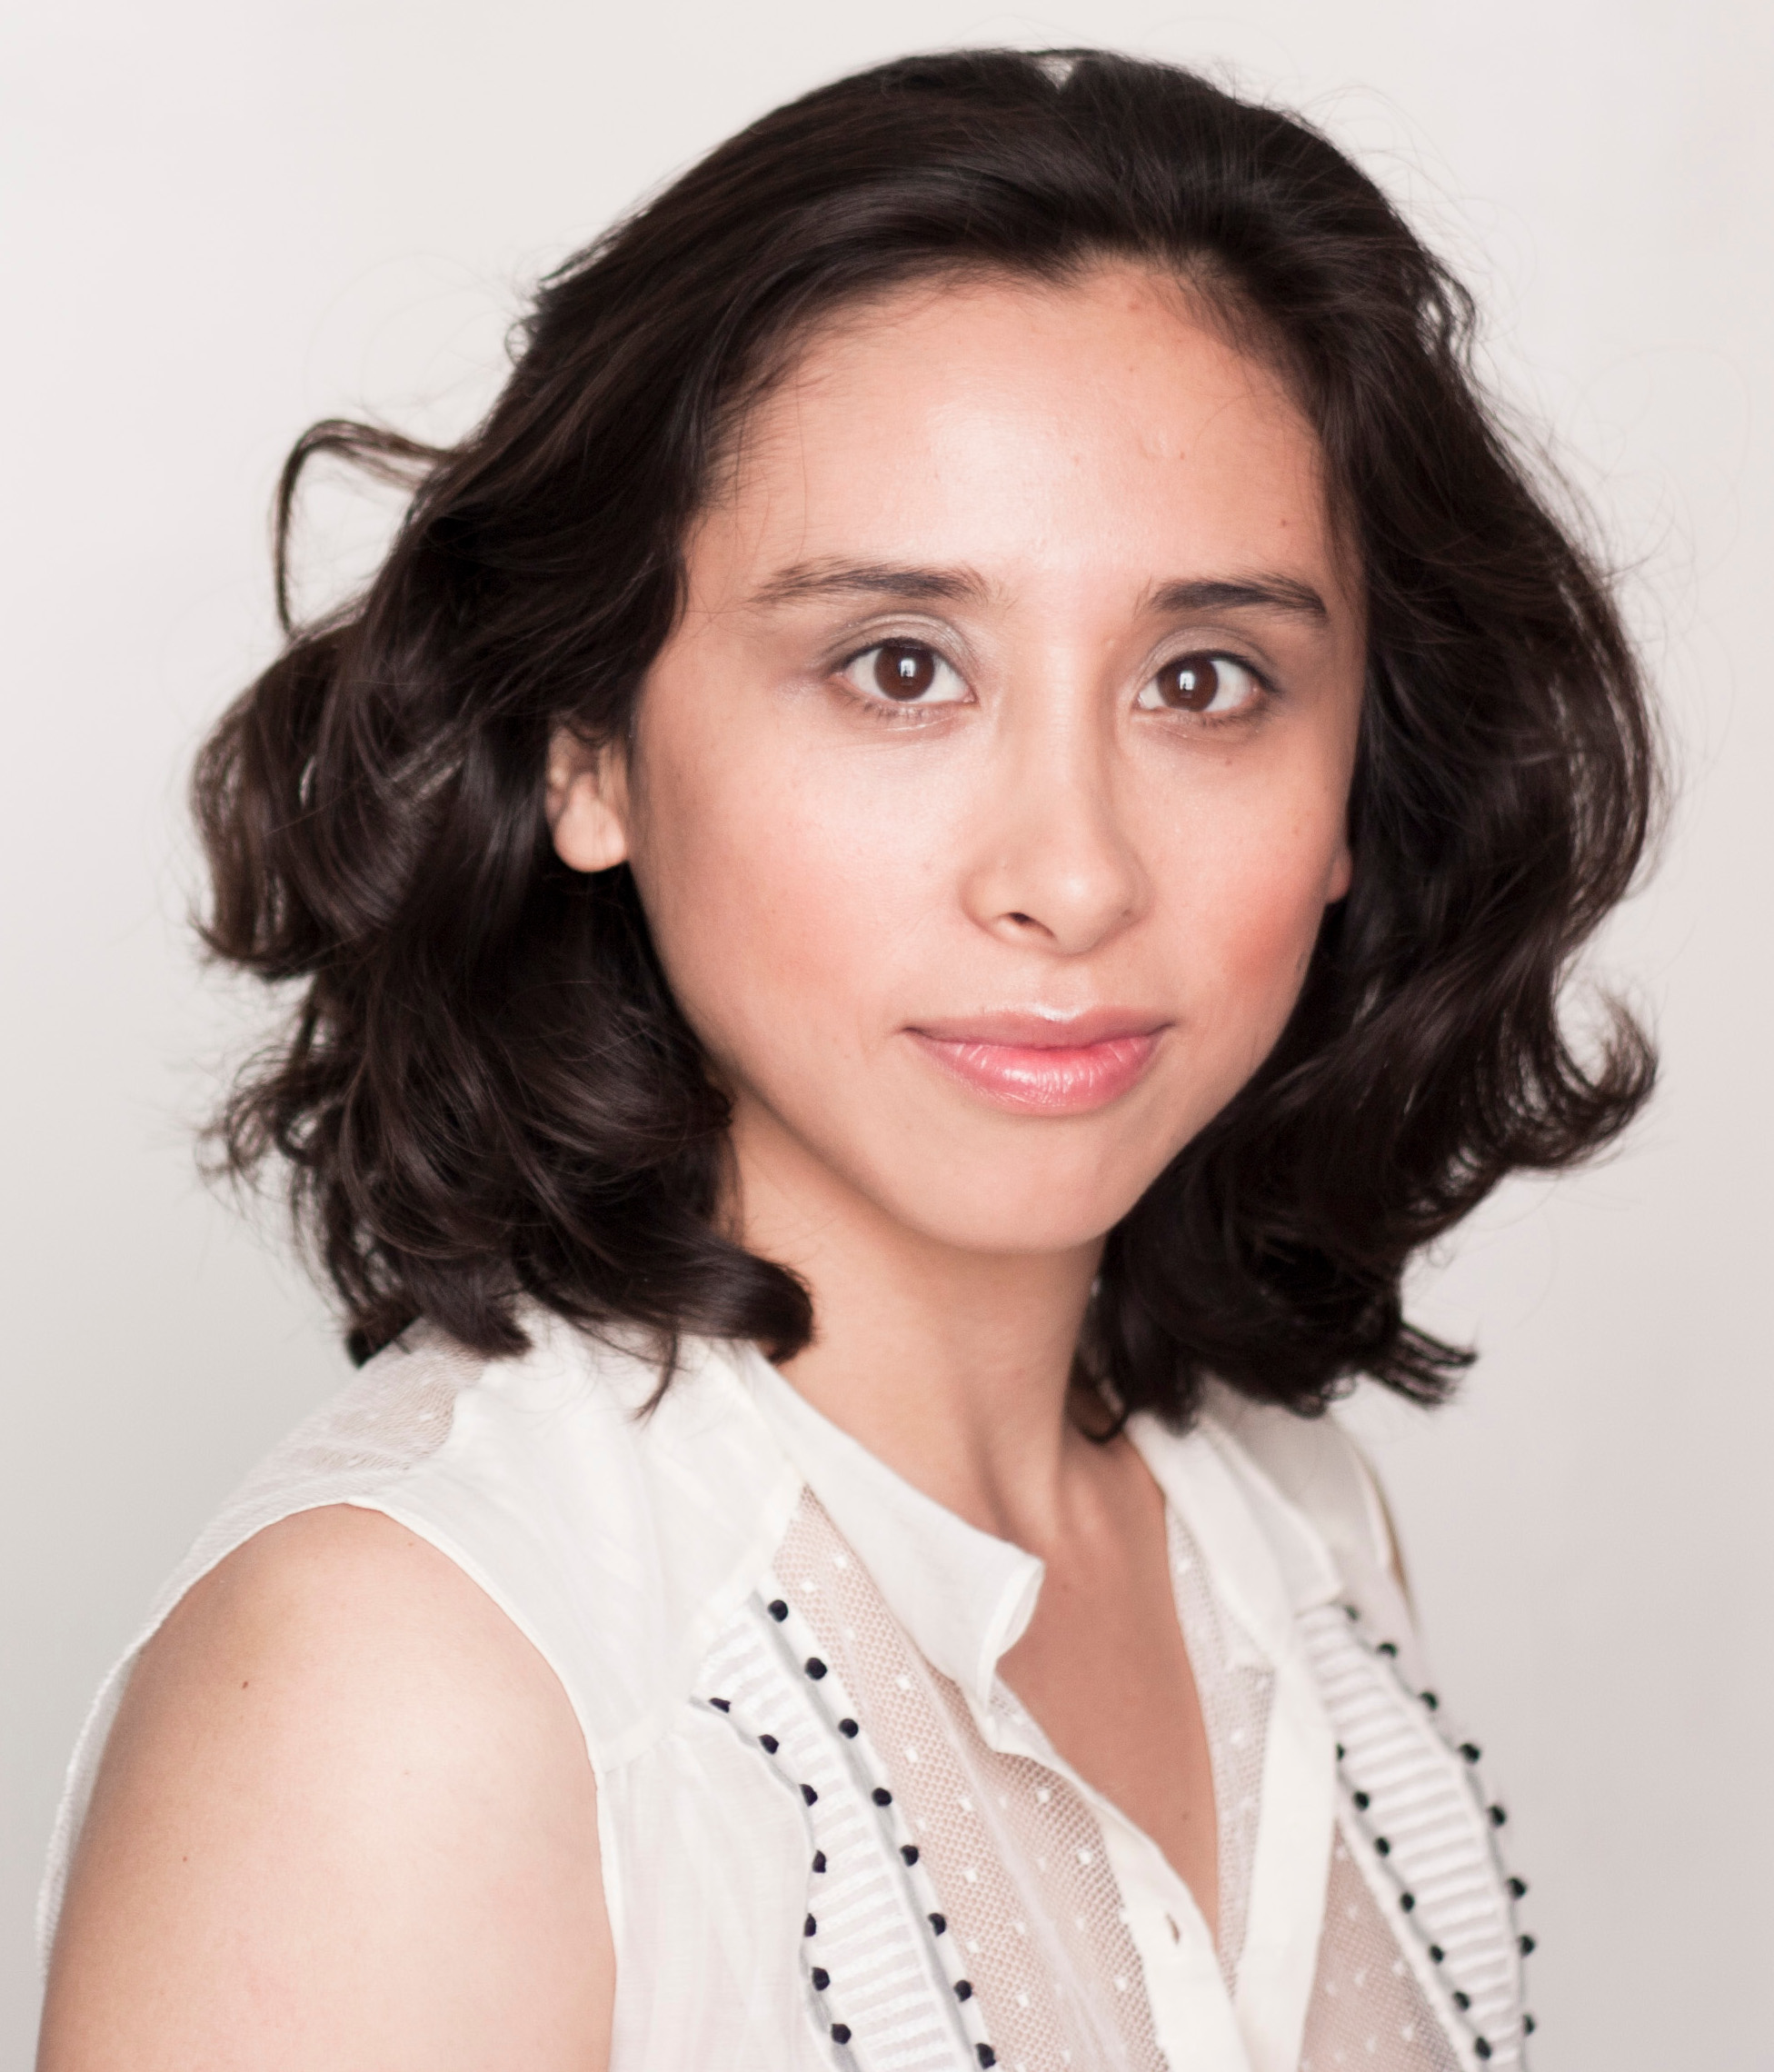
\includegraphics[width=.3\textwidth]{pili_big3.jpg} \\
\end{tabular}

\renewcommand{\tabcolsep}{0.4cm}

\renewcommand{\arraystretch}{1.5}
%\section*{Other training}
%\vspace{-0.3cm}

\subsection*{Theatre}
\vspace{-0.3cm}
\begin{five_col}
  2015
  & The Man Who Was Thursday
  & Mask creation and mask-play direction
  & The Provisional Players
  & Oliver Schroeder \\

  2014
  & The Affair
  & Female Lead 2 (Woman 2)
  & Les Fanatic \& Presentimental
  & \pbox{5cm}{Amy Gibbons \& \\ Samuel Gaulier} \\[0.25cm]

  2011
  & Watership Down
  & General Woundwort
  & Alles is Drama
  & Sybrand van der Werf \\

  2011
  & The Vagina Monologues
  & Ensemble
  & Queer it up
  & Anna in't Veld \\[0.25cm]

  2010
  & S\'{o}lo la brisa del mundo puede tocar la flor de nuestras cabezas
  & Presenter/Dancer
  & TOT Cultural Association
  & \pbox{5cm}{Oscar Betancourt \& \\ Pilar Andrea Quiroz} \\

  2009
  & Muerte (una comedia)
  & Rebeca
  & TOT Cultural Association
  & Oscar Betancourt \\

\end{five_col}

\begin{five_col}

  2009
  & Entre desvar\'{i}os y piezas rotas
  & Woman
  & TOT Cultural Association
  & Oscar Betancourt \\

  2008
  & Prohibido suicidarse en primavera
  & Hans
  & TOT Cultural Association
  & Oscar Betancourt \\

\end{five_col}

\subsection*{Performance}
\begin{five_col}
  2011
  & Kas
  & Girl
  & Alles is Drama
  & Marijn Alexander de Jong \\

  2010
  & Locura suspendida
  & Ensemble, acrobalance
  & Ubuntu
  & Collective creation \\

  2010
  & Cuerpos deshechos
  & Ensemble, acrobalance
  & Ubuntu
  & Collective creation \\

  2010
  & Conflicto. Equilibrios y tensiones
  & Ensemble, acrobalance
  & Ubuntu
  & Collective creation \\

\end{five_col}

\subsection*{Film}
\begin{five_col}
  2014
  & Music video \href{https://www.youtube.com/watch?v=bFKCZNJZVbY}{``It's easy to say'' by Blanche}
  & Mime
  &
  & \pbox{5cm}{Alexander J.E. Bradley \& \\ Anni Maarit} \\
\end{five_col}

% \section*{Special Skills}
% \begin{tabular}{p{3.3cm}p{12cm}}
%   Sports
%   & Swimming, roller skating \\

%   Languages
%   & Spanish (native), English, French \\

%   Acrobatics
%   & Aerial acrobatics (silks)
% \end{tabular}

\subsection*{Workshops}
\begin{three_col}
  2015
  & Polichinelo Circus, Liverpool
  & 8 weeks intensive, Acrobatics Course \\

  2010
  & La Ventana Producciones, Colombia
  & 2 weeks intensive, Aerial Acrobatics Workshop \\

  2010
  & Buenavista Social Clown, Colombia
  & 2 weeks intensive, Commedia dell'arte and leather mask sculpting workshop \\

  2009
  & La Instalacción Escuela de Circo y Danza, Argentina
  & 4 weeks intensive, Aerial Acrobatics training \\
\end{three_col}


\end{document}
